\setcounter{chapter}{15}% Equivalent to "letter O"
\renewcommand{\thechapter}{\Alph{chapter}}
\Chapter{An�lisis de resultados}

\justify
\section{An�lisis correlacional}

El an�lisis de las variable de muestra que existe una relaci�n entre la satisfacci�n de la carrera y la elecci�n de carrera, esta correlaci�n  provee un indice de Pearson de  0.88.  Esto demuestra que existe una correlaci�n positiva entre ambas variables de inter�s

\begin{table}[H]
	\begin{center}
		\caption{Correlaci�n de Pearson entre satisfacci�n en la carrera y la elecci�n de la misma}
		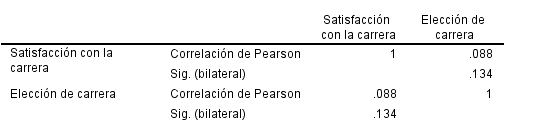
\includegraphics[scale=0.95]{ANA_CORRE_IMG1}
	\end{center}
\end{table}

\justify
\section{Edad de los estudiantes encuestados}
A continuaci�n se presenta la gr�fica donde se muestra la distribuci�n por edad de las personas entrevistadas.\\

\begin{figure}[H]
	\begin{center}
		\caption{Distribuci�n de personas encuestadas seg�n su edad.}
		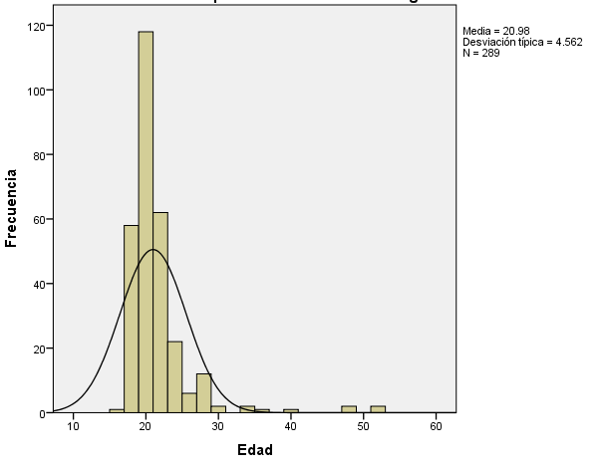
\includegraphics[scale=0.95]{edades}
	\end{center}
\end{figure}

Se encontr� que aproximadamente el 50\% de las personas que fueron encuestadas se encontraba en un rango de 19 a 22 a�os, con una media de edad de 21 a�os y teniendo casos at�picos.\\

\begin{table}[H]
	\begin{center}
		\caption{Frecuencia de estudiantes que presentan el deseo de haber seguido otra carrera seg�n su rango de edad.}
		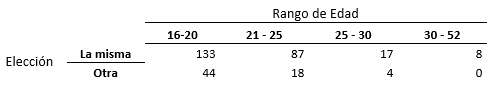
\includegraphics[scale=0.95]{edad-deseo}
	\end{center}
\end{table}

En el cuadro se muestra que las personas que son m�s j�venes en edad deseaban haber escogido otra carrera, y que este n�mero  fue disminuyendo conforme aumentaba la edad de los encuestados. Lo que muestra, es que mientras m�s joven era la persona encuestada era m�s probable que la persona no quisiera cambiarse de carrera, aunque hab�a posibilidad de que prefiriera otra carrera. Sin embargo al aumentar la edad del encuestado no hab�a duda de que el encuestado cada vez m�s no consideraba elegir alguna otra carrera.\\


\section{Sexo de los estudiantes encuestados}
La gr�fica de sectores que se muestra a continuaci�n muestra que las personas encuestadas para esta investigaci�n eran en su mayor�a de sexo femenino representando un 55.71\% de la muestra total encuestada y el sexo masculino el 44.29\% restante de la muestra.\\

\begin{figure}[H]
	\begin{center}
		\caption{Proporci�n de la muestra encuestada seg�n su sexo.}
		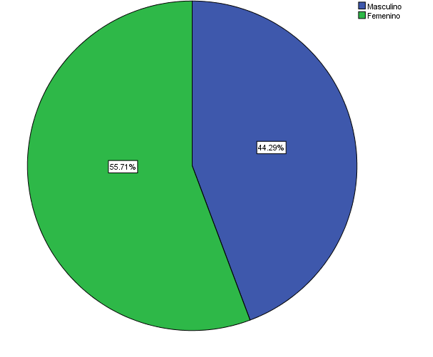
\includegraphics[scale=0.95]{genero}
	\end{center}
\end{figure}

El cuadro O.1 muestra la cantidad de hombres y de mujeres que hubieran preferido seguir otra carrera y los que prefieren la carrera que cursan. De las 161 mujeres que fueron encuestadas el 23.60\%, es decir 38 mujeres, hubieran preferido seguir otra carrera de no ser por factores externos que influenciaron en su decisi�n. Por otro lado, de los 128 hombres que fueron encuestados el 21.87\%, es decir 28 hombres, hubieran preferido cursar otra carrera de no ser por los factores externos que pudieron influenciar en su decisi�n\\

\begin{figure}[H]
	\begin{center}
		\caption{Proporci�n de la muestra encuestada seg�n su sexo.}
		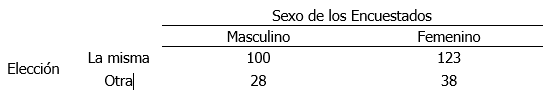
\includegraphics[scale=0.95]{sexo-cambio}
	\end{center}
\end{figure}


